\documentclass[10pt,a4paper]{article}
\usepackage[margin=0.8in]{geometry}
\usepackage[T1]{fontenc}
\usepackage{graphicx,microtype,float}
\usepackage{xurl}
\usepackage[hidelinks]{hyperref}
\hypersetup{pdfauthor={Anonymous authors},pdftitle={Jira Enhancer: Supplementary Figure S2 -- Matched-Review Radar Plot},pdfsubject={Human-rated requirement dimensions and priority-weighted composite scores}}
\pdfinfoomitdate=1
\pdftrailerid{}
\raggedbottom
\emergencystretch=1.5em
\renewcommand{\thefigure}{S\arabic{figure}}
\setcounter{figure}{1}
\begin{document}
\begin{center}
\Large Jira Enhancer: Supplementary Matched-Review Radar Plot\\[0.4em]
\normalsize Anonymous authors
\end{center}

\begin{figure}[H]
\centering
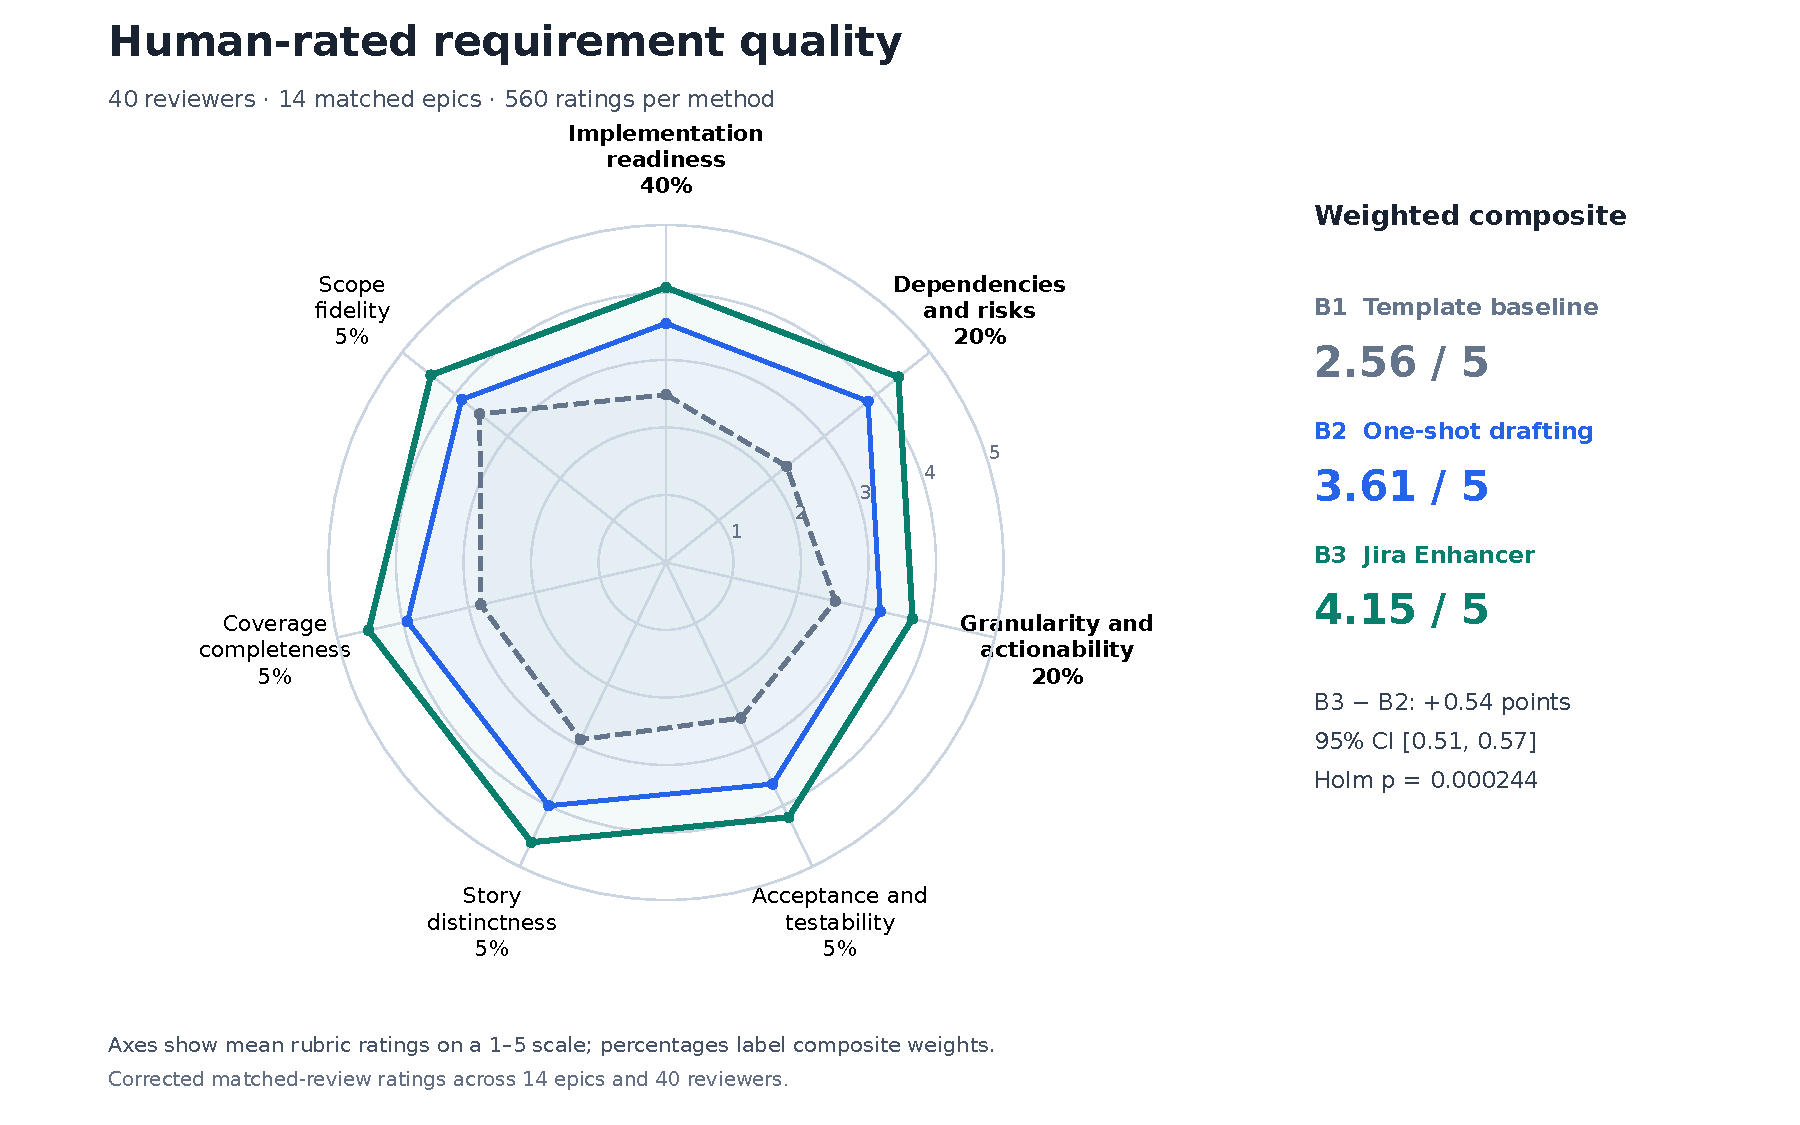
\includegraphics[width=\linewidth]{../patent/reviewer_study/public_results/matched_review_weighted_radar.pdf}
\caption{Human-rated requirement quality for B1 (template baseline), B2 (one-shot drafting), and B3 (Jira Enhancer). The radar shows mean ratings for seven requirement dimensions on the anchored 1--5 scale. Percentages beside the axes are the weights used for the priority composite shown on the right; the radar points show the dimension means before weighting.}
\label{fig:supp-matched-review-radar}
\end{figure}

\paragraph{Study and interpretation.}
The figure uses the corrected matched-review data from 40 reviewers and 14 epic packages per method, giving 560 primary package ratings for each method. The 160 masked-repeat ratings are excluded. B3 uses RL-guided prompt selection and bounded refinement. It has higher mean ratings on all seven dimensions. Implementation readiness receives 40\% of the composite weight; dependencies and risks and granularity and actionability receive 20\% each; the other four dimensions receive 5\% each.

The priority-weighted means are 2.56 for B1, 3.61 for B2, and 4.15 for B3. The B3--B2 paired difference is +0.54 points, with a 95\% epic-bootstrap confidence interval of [0.51, 0.57] and Holm-adjusted exact paired sign-flip $p=0.000244$. The 14 matched epics are the units of inference, and the Holm adjustment covers the two declared baseline contrasts. These are the same results reported in Section 5.3 of the main manuscript. The equal-weight comparison is also reported there and in \href{https://github.com/anonymous94u/JiraEnhancer/blob/main/supplementary/appendices_a_b.pdf}{Supplementary Appendix B}.

\paragraph{Data and reproduction.}
The original graphic is retained unchanged. Its inputs are the public \href{https://github.com/anonymous94u/JiraEnhancer/blob/main/patent/reviewer_study/public_results/matched_review_quality_factor_comparison.csv}{dimension means and weights}, \href{https://github.com/anonymous94u/JiraEnhancer/blob/main/patent/reviewer_study/public_results/matched_review_method_summary.csv}{method summaries}, and \href{https://github.com/anonymous94u/JiraEnhancer/blob/main/patent/reviewer_study/public_results/matched_review_pairwise.csv}{paired comparisons}. The \href{https://github.com/anonymous94u/JiraEnhancer/blob/main/patent/reviewer_study/plot_weighted_review_radar.py}{plotting script} and \href{https://github.com/anonymous94u/JiraEnhancer/blob/main/patent/reviewer_study/public_results/matched_review_weighted_radar.pdf}{original vector PDF} are available in the same repository.
\end{document}
